\documentclass[conference]{IEEEtran}
\IEEEoverridecommandlockouts
% The preceding line is only needed to identify funding in the first footnote. If that is unneeded, please comment it out.
\usepackage{cite}
\usepackage{amsmath,amssymb,amsfonts}
\usepackage{algorithmic}
\usepackage{graphicx}
\usepackage{textcomp}
\usepackage{xcolor}
\def\BibTeX{{\rm B\kern-.05em{\sc i\kern-.025em b}\kern-.08em
    T\kern-.1667em\lower.7ex\hbox{E}\kern-.125emX}}

\usepackage{subfigure}    
\begin{document}

\title{Comaparative Analysis of the Non-Local Algorithm for Image Restoration with Previous Techniques}

\author{\IEEEauthorblockN{J. Serdoncillo}
\IEEEauthorblockA{\textit{EE 5561: Image Processing and Applications} \\
\textit{University of Minnesota - Twin Cities \\
Minneapolis, United States \\
serdo004@umn.edu} }}

\maketitle

\begin{abstract}
Denoising methods that are most commonly used are of the neighborhood filtering techniques or simple averaging filters. In this paper, we implement 
and explore patch-based similarity within a single image through the use of non-local means. Non-local means work by taking a weighted average based 
on similarity. The paper claims that this creates a fairly fast method which is able to perform significantly better than other current methods.
 The method is implemented using python and will be compared with different denoising techniques for both gaussian and salt n' pepper noise to prove the
 effectiveness of the non-local algorithm. The paper concludes with a table of results of performance metrics using PSNR and MSE compared with previous methods. 
 Additionally, an exploration of the hyperparameters was shown to produce different results.
\end{abstract}

\begin{IEEEkeywords}
Image Denoising, Non-Local Means, Patch-based method
\end{IEEEkeywords}

\section{Introduction}
\subsection{Denoising Techniques}
%% relate this based on the papers we have
%% relate this based on the lectures
Image denoising methods have been really important in the field of imaging. The main goal of image denoising is to be able to recover the most accurate
representation of the image from a noisy measurement that could be caused by the measurement apparatus or the environment itself. During the previous lectures,
the main denoising methods that have been learned have been the gaussian smoothing model \cite{gf} which is makes the image look better but we lose some of the features, 
the mean filtering \cite{mf} which is particularly great for removing salt and pepper noise, and the total variation diminishing methods \cite{tvd} using proximal gradient descent 
or alternating direction method of multipliers method which converges to the the real value but is limited with the amount of computation and number of iterations 
needed for a satisfying result. These methods are the main methods that have been learned which can be applied to a singular image. 
Aside from the methods mentioned above, there are also averaging methods that can be used if multiple snapshots of the same image \cite{ave} can be gathered which can give 
a really great result. 

This one can be attributed to a "patch-based" method which is the similarity between whole images \cite{source}. Taking the same technique but for similarity wi
within the image itself, the similar signal content can be taken advantaged off to have a weighted average of similar patches around a singular area which was summarized
as "through-time" averaging on a single image. Of course, this method might not work for all types of images because there might not be much similarity but it is worth trying
which covers the scope of this paper.

\section{Methodology}
\subsection{Noise Implementation}
The two types of noise will be used in this paper, gaussian noise and salt and pepper noise \cite{mf}. Gaussian noise was added by choosing a mean and standard deviation
which will then be used to form the gaussian noise which can be added to the following image \cite{g}. On the other hand, the salt and pepper noise was implemented by prescribing
a concentration of salt and pepper noise and random locations within the image were changed to 255 and 0 respectively.

\subsection{Non-Local Means Implementation}
%% Read about in the paper
To implement the non-local means denoising method, the estimated value of the output image for a certain pixel is computed as a weighted averageof all of the pixels in the image
as seen in the equation below. The weights are dependent on the similarity between pixels $i$ and $j$ and should sum up to 1 \cite{source}.

\begin{equation}
    \mathbf{\hat{x}} = \sum_{j \in I}w(i,j)\mathbf{v}(j)
\end{equation}

The weights are calculated as the similarity between the square neighborhood of two different pixels baesd on the weighted Euclidean distance.
Higher similarities are given higher weights while lower similarties are given lower weights. Overall, the equation for the weights are as shown below and a normalizing constant definition
as well.

\begin{figure}[htbp]
    \centering
    \subfigure[]{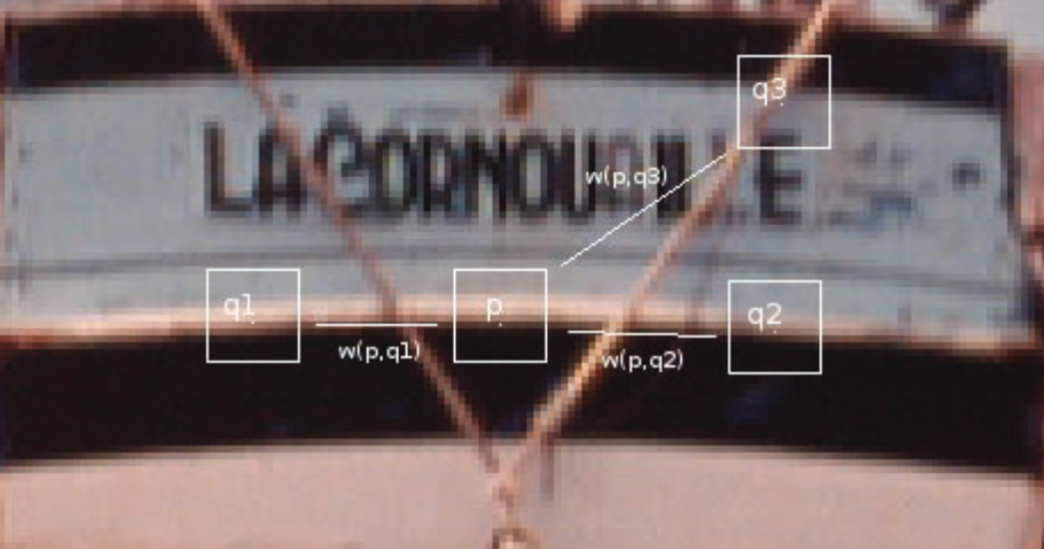
\includegraphics[width=0.40\textwidth]{images/paper/nl1.png}}
    \caption{Similarity windows for self-similarity \cite{review}}
\end{figure}

\begin{equation}
    w(i,j) = \frac{1}{Z(i)}e^{\frac{||v(N_i)-v(N_j)||_2^2}{h^2}}
\end{equation}

\begin{equation}
    Z(i) = \sum_{j} e^{\frac{||v(N_i)-v(N_j)||_2^2}{h^2}}
\end{equation}

\begin{figure}[htbp]
    \centering
    \subfigure[]{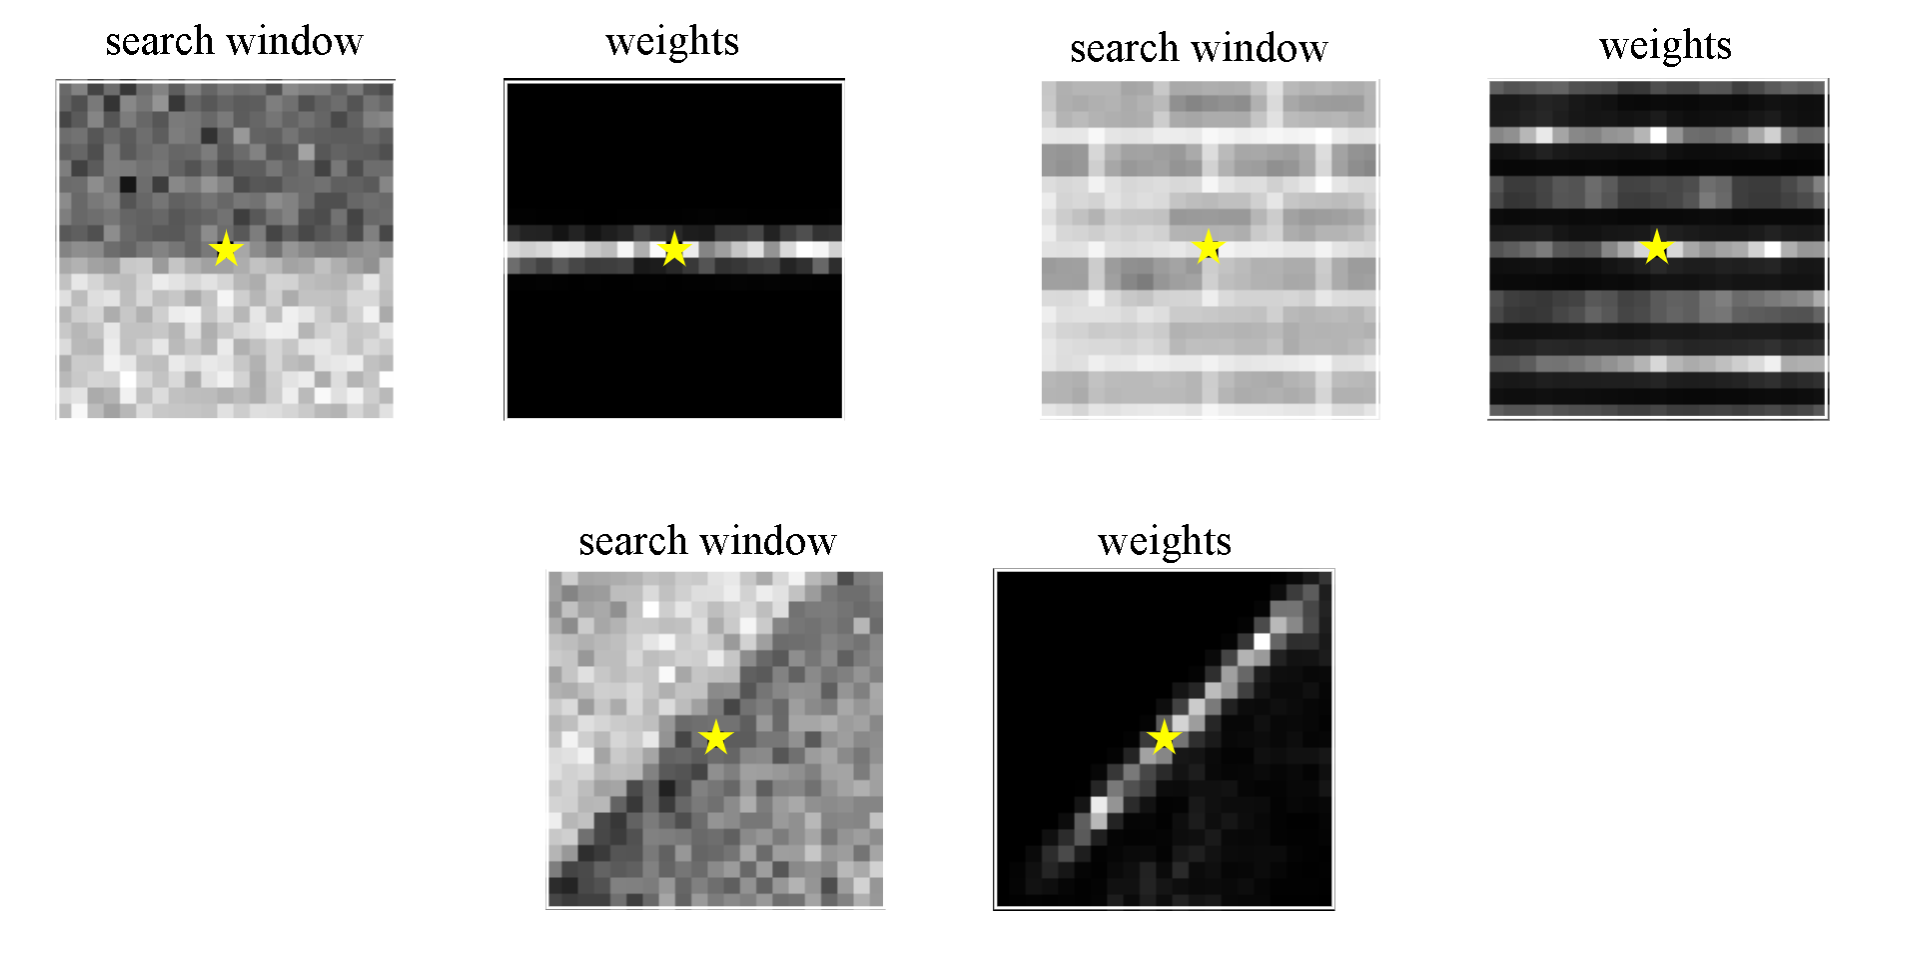
\includegraphics[width=0.40\textwidth]{images/paper/w.png}}
    \caption{Weights using non-local means \cite{source}}
\end{figure}

The reason why a neighborhood is chosen is so that there is a penalization between similar pixel intensity values but not it's neighbors and at the same time
having a reward for having a similar neighborhood but not the same intensity value of the specific pixel. It can already be seen now that this method works well n
not only with gaussian noise but also with salt and pepper noise as well.
Finally, the weighted average is repeated for all of the pixel values in the neighborhood until the solution converges to a valid result.

\section{Results}

    To start with testing the new denoising method, the following common images are used for the results and analysis which are photos that were used in the previous homeworks.
    These are the lena image, man image, coins, and the cameraman image. The original image will be used to manually introduce both the gaussian and, salt and pepper noise.
    For the sake of time and computational power, all of the images were scaled and cropped to form a 200 by 200 image resolution.

    \begin{figure}[htbp]
        \centering
        \subfigure[]{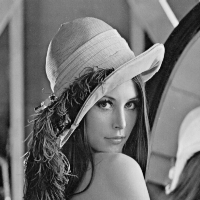
\includegraphics[width=0.2\textwidth]{images/lena5120.png}}
        \subfigure[]{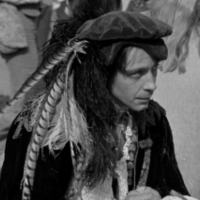
\includegraphics[width=0.2\textwidth]{images/man0.png}}
        \subfigure[]{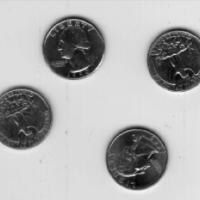
\includegraphics[width=0.2\textwidth]{images/eight0.png}}
        \subfigure[]{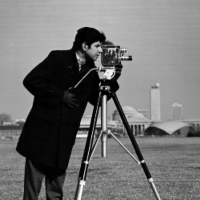
\includegraphics[width=0.2\textwidth]{images/cameraman0.png}}
        \caption{Common Images used for testing (a) lena (b) man (c) coins (d) cameraman}
    \end{figure}

    The following images below are the gaussian noise prescribed with a mean of 0 and variance of 500. It is noted that the pixel values are in the range of 0 to 255, hence the large variance value.

    \begin{figure}[htbp]
        \centering
        \subfigure[]{\includegraphics[width=0.2\textwidth]{images/noised/g0.png}}
        \subfigure[]{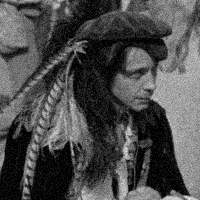
\includegraphics[width=0.2\textwidth]{images/noised/g1.png}}
        \subfigure[]{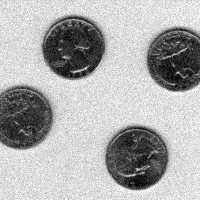
\includegraphics[width=0.2\textwidth]{images/noised/g2.png}}
        \subfigure[]{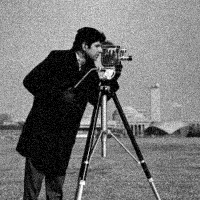
\includegraphics[width=0.2\textwidth]{images/noised/g3.png}}
        \caption{Gaussian Noise for the images of (a) lena (b) man (c) coins (d) cameraman}
    \end{figure}

    On the other hand, the following images below are the final images with the salt and pepper noise applied. These were prescribed with a salt and pepper probability of 1\% for both.

    \begin{figure}[htbp]
        \centering
        \subfigure[]{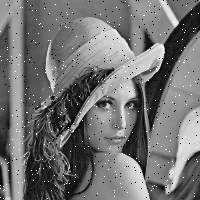
\includegraphics[width=0.2\textwidth]{images/noised/s0.png}}
        \subfigure[]{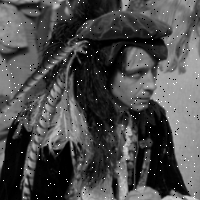
\includegraphics[width=0.2\textwidth]{images/noised/s1.png}}
        \subfigure[]{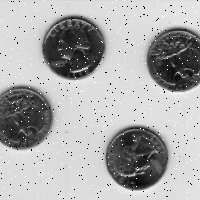
\includegraphics[width=0.2\textwidth]{images/noised/s2.png}}
        \subfigure[]{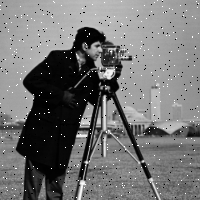
\includegraphics[width=0.2\textwidth]{images/noised/s3.png}}
        \caption{Salt and Pepper Noise for the images of (a) lena (b) man (c) coins (d) cameraman}
    \end{figure}

    In implementing the non-local means algorithm, similar hyperparameters were chosen as with the original paper with a square neighborhood size of 7, 
    search neighborhood size of 21 but a last h value which is equal to 10. The following qualitative results upon running the algorithm is as shown in the figures below which
    is only applied to the gaussian noise. Despite the high amounts of noise added to the original image, it can be seen that the non-local means algorithm performs pretty well. 
    and is able to remove some of the noise while keepig the amount of detail.

    \begin{figure}[htbp]
        \centering
        \subfigure[]{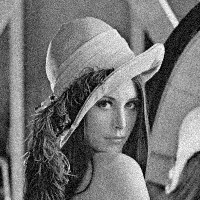
\includegraphics[width=0.2\textwidth]{images/denoised/gnl0.png}}
        \subfigure[]{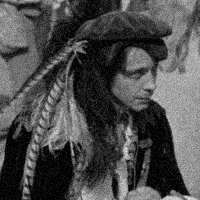
\includegraphics[width=0.2\textwidth]{images/denoised/gnl1.png}}
        \subfigure[]{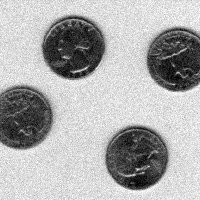
\includegraphics[width=0.2\textwidth]{images/denoised/gnl2.png}}
        \subfigure[]{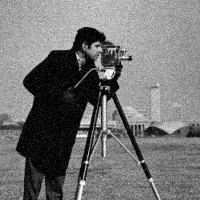
\includegraphics[width=0.2\textwidth]{images/denoised/gnl3.png}}
        \caption{NonLocal Means Denoising for the images of (a) lena (b) man (c) coins (d) cameraman}
    \end{figure}

\section{Discussion}

\subsection{Comaparative Peformance}
%% Talk about what other methods we will compare it with
%% Talk about the metrics that we will be using
    To compare the performance of the different methods, two different types of metrics are used which are the peak signal to noise ratio (PSNR) and the mean squared error (MSE).
    A higher value of PSNR means a lower noise ratio and a lower value of MSE means a lower deviation from the actual image. This means that the ideal value would be an infinite PSNR 
    and a 0 MSE. In the tables below, the before and after values for both the PSRN and MSE are shown. The various different methods that were also learned in class are as shown which are 
    the gaussian filter (GF), median filter (MF), total variation diminishing using proximal gradient descent (TVD1) and the the total variation diminishing using alternating direction multiplier method (TVD2).
    Lastly the performance of the nonlocal (NL) is shown in the last column to easily see how it performs compared to the previous methods. 
    All of the methods are also applied to the two types of noise. It is to be noted that due to the high value of noise added to the system, a lower value for the variance of the gaussian noise is lower for NL
    which is now changed to 160. This is because there were large error values that were noted. To have a similar implementation as the papers, a square window of 7, search window of 21 and h of 10 was used. 

    \begin{table}[htbp]
    \caption{PSNR table for Gaussian Noise}
    \begin{center}
    \begin{tabular}{|c|c|c|c|c|c|}
    \hline
    \textbf{}&\multicolumn{5}{|c|}{\textbf{Denoising Methods}} \\
    \cline{2-6} 
    \textbf{Image} & \textbf{\textit{GF}}& \textbf{\textit{MF}}& \textbf{\textit{TVD1}} & \textbf{\textit{TVD2}} & \textbf{\textit{NL}} \\
    \hline
    Lena &21-25&21-25&21-6&21-6 & 21- \\
    \hline
    Man &20-26&20-25&20-7&20-7 &20-  \\
    \hline
    Coins &21-28&21-27&21-2&21-2 &21-  \\
    \hline
    Cameraman&22-26&25-26&21-6&21-6 &22-  \\
    \hline
    \end{tabular}
    \label{tab1}
    \end{center}
\end{table}

The tables above with the gaussian noise clearly shows the effectiveness of the gaussian and median filter with similar increases for PSNR. The values for the TVD methods are as is because a lower value for iterations was used which
produced below average qualities for denoising. It is to be noted however that previous implementations of the TVD methods in the previous homeworks were working and was not fixed in this paper due to time constraints.
It can be seen that the gaussian filter outperforms the median filter by a bit. This can be due to the size of the gaussian filter compared with the median filter.
    \begin{table}[htbp]
        \caption{MSE table for Gaussian Noise}
        \begin{center}
        \begin{tabular}{|c|c|c|c|c|c|}
        \hline
        \textbf{}&\multicolumn{5}{|c|}{\textbf{Denoising Methods}} \\
        \cline{2-6} 
        \textbf{Image} & \textbf{\textit{GF}}& \textbf{\textit{MF}}& \textbf{\textit{TVD1}} & \textbf{\textit{TVD2}} & \textbf{\textit{NL}} \\
        \hline
        Lena &482-168&479-184&487-16204&487-16204 &485  \\
        \hline
        Man &438-105&434-125&443-8621&443-8621 &444  \\
        \hline
        Coins &461-88&465-130&452-34896&452-34896 &459  \\
        \hline
        Cameraman &450-160&452-168&454-17236&454-17236 &448  \\
        \hline
        \end{tabular}
        \label{tab1}
        \end{center}
    \end{table}

    \begin{table}[htbp]
        \caption{PSNR table for SnP Noise}
        \begin{center}
        \begin{tabular}{|c|c|c|c|c|c|}
        \hline
        \textbf{}&\multicolumn{5}{|c|}{\textbf{Denoising Methods}} \\
        \cline{2-6} 
        \textbf{Image} & \textbf{\textit{GF}}& \textbf{\textit{MF}}& \textbf{\textit{TVD1}} & \textbf{\textit{TVD2}} & \textbf{\textit{NL}} \\
        \hline
        Lena &22-26&22-28&21-5&21-5 &21  \\
        \hline
        Man &20-27&20-32&20-7&20-7 &20  \\
        \hline
        Coins &21-28&21-32&21-2&21-2 & 21 \\
        \hline
        Cameraman&22-26&22-29&22-6&22-6 &22  \\
        \hline
        \end{tabular}
        \label{tab1}
        \end{center}
    \end{table}

    In terms of the tables for salt and pepper noise, it can be seen now that the median filter outperforms the gaussian filter which is what it is mainly used for. 

    \begin{table}[htbp]
        \caption{MSE table for SnP Noise}
        \begin{center}
        \begin{tabular}{|c|c|c|c|c|c|}
        \hline
        \textbf{}&\multicolumn{5}{|c|}{\textbf{Denoising Methods}} \\
        \cline{2-6} 
        \textbf{Image} & \textbf{\textit{GF}}& \textbf{\textit{MF}}& \textbf{\textit{TVD1}} & \textbf{\textit{TVD2}} & \textbf{\textit{NL}} \\
        \hline
        Lena &378-164&409-82&382-16204&382-16204 &391  \\
        \hline
        Man &420-93&448-31&437-8621&437-8621 &427  \\
        \hline
        Coins &458-94&443-34&466-34896&466-34896 &473  \\
        \hline
        Cameraman&399-157&415-79&401-17236&401-17236 &393  \\
        \hline
        \end{tabular}
        \label{tab1}
        \end{center}
    \end{table}

    Overall it can be seen that a somewhat failed implementation of the nonlocal means algorithm was done in addition to the bugs from the TVD methods.
    It is to be noted however that the jumps aren't as big as before.


        
\subsection{Hyperparameter Tweaking}
Tweaking the hyperparameters of the nonlocal denoising method can significantly impact the quality of the denoised image. The three main hyperparameters are the square window size, the search window size, and the parameter h.

The square window size determines the size of the local neighborhood around each pixel that is used for denoising. A larger square window size can help to preserve larger structures in the image, but it may also blur fine details.

The search window size determines the range of pixels that are considered when searching for similar patches in the image. A larger search window size can help to find more similar patches, especially in textured or repetitive regions of the image. However, it also increases the computational complexity of the algorithm.

The parameter h controls the decay of the Gaussian function used for weighting the patches in the image. A larger h value gives more weight to distant patches, which can help to reduce noise but may also blur the image.

Therefore, these hyperparameters should be carefully tuned based on the specific characteristics of the input image and the desired trade-off between noise reduction and preservation of image details. It’s often beneficial to experiment with different settings and evaluate the results visually or using objective image quality metrics.

In the table below, different combinations of the hyperparameters are chosen to produce the denoised images below.
    \begin{figure}[htbp]
        \centering
        \subfigure[]{\includegraphics[width=0.13\textwidth]{images/hyper/g0.png}}
        \subfigure[]{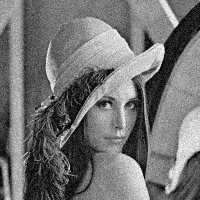
\includegraphics[width=0.13\textwidth]{images/hyper/g1.png}}    
        \subfigure[]{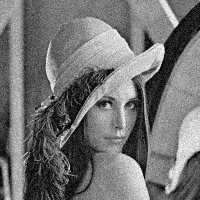
\includegraphics[width=0.13\textwidth]{images/hyper/g2.png}}
        \subfigure[]{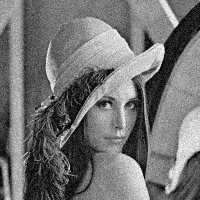
\includegraphics[width=0.13\textwidth]{images/hyper/g3.png}}
        \subfigure[]{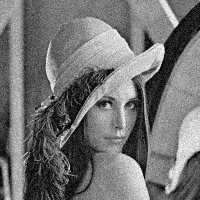
\includegraphics[width=0.13\textwidth]{images/hyper/g4.png}}
        \subfigure[]{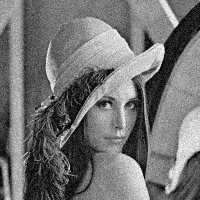
\includegraphics[width=0.13\textwidth]{images/hyper/g5.png}}
        \caption{NonLocal Means Denoising for the images of lena with various hyperparameters}
    \end{figure}
The metrics for their effectiveness is as shown in the figure below. It can be seen that the change in the hyperparameters greatly affects the performance is is hard to find 
what the ideal combination is beforehand and especially if one does not know anything about the noise.
    \begin{table}[htbp]
        \caption{Metric Table for Hyperparameter tweaking}
        \begin{center}
        \begin{tabular}{|c|c|c|c|c|}
        \hline
        \textbf{Square} & \textbf{Search} & \textbf{h} & \textbf{\textit{PSNR}} & \textbf{\textit{MSE}} \\
        \hline
        7 & 21 & 10 & & \\
        \hline
        7 & 21 & 5 & & \\
        \hline
        3 & 21 & 10 & &  \\
        \hline
        3 & 13 & 5 & & \\
        \hline
        5 & 17 & 7 & & \\
        \hline
        \end{tabular}
        \label{tab1}
        \end{center}
    \end{table}

\section{Conclusions}
    Aside from the usual methods for denoising, self-similarity between and within images has been shown to produce substantial results despite the simpleness of their algorithms.
    And as seen in the previous papers which were the basis of this paper, the non-local means algorithm is able to perform significantly better results based on the mean-squared error metric.
    Although it was also mentioned that the numerical measurement might not be most objective one not is it representation of a higer visual quality. In this paper, more metrics were used and images were shown which
    might convince the reader better with its effectiveness.

    \subsection{Limitations}
    The non-local means algorithm although great in paper has some similar limitations as compared with the mini project 1 paper that was discussed. The main issues with these are the denoising of pixels one at a time which
    can be time and computationally consuming. At the same time, there are lots of hyperparameters that can be tweaked which might produce different qualities of results and might not even be consistent across different sets of noises or images. 
    Lastly, one thing that would be worth mentioning which was not talked in the previous papers is it's possible performance for images which have poor self-similarity between any of the patches. It might be hard to visualize of such a thing but 
    is still not impossible especially for images with high amounts of detail but no pattern nor noisy abstraction.

    \subsection{Future Work}
    With regards to the success of the non-local means algorithm, more can still be done due to the limitaion of the prescribed search window. 
    Instead of searching for similar patches in the neighborhood, the patch can be taken from the whole image which can be calculated efficiently 
    through the use of convolutions. Having a cutoff for the chosen patches can also be done which can make sure that non-similar images can be disregarded instead.

\section*{Acknowledgment}
The author would like to thank Professor Akcakaya and Merve Gulle for showing me the new world in image processing and the wonders contained in it.  

\begin{thebibliography}{00}
\bibitem{source} Buades, Antoni, Bartomeu Coll, and J-M. Morel. "A non-local algorithm for image denoising." 2005 IEEE computer society conference on computer vision and pattern recognition (CVPR'05). Vol. 2. Ieee, 2005.

\bibitem{review} Buades, Antoni, Bartomeu Coll, and Jean-Michel Morel. "Image denoising methods. A new nonlocal principle." SIAM review 52.1 (2010): 113-147.

\bibitem{gf} Lindenbaum, M., Fischer, M., & Bruckstein, A. (1994). On Gabor's contribution to image enhancement. Pattern recognition, 27(1), 1-8.

\bibitem{tvd} Rudin, L. I., Osher, S., & Fatemi, E. (1992). Nonlinear total variation based noise removal algorithms. Physica D: nonlinear phenomena, 60(1-4), 259-268.

\bibitem{g} Slepian, D. (1962). The one‐sided barrier problem for Gaussian noise. Bell System Technical Journal, 41(2), 463-501.

\bibitem{mf} Chan, R. H., Ho, C. W., & Nikolova, M. (2005). Salt-and-pepper noise removal by median-type noise detectors and detail-preserving regularization. IEEE Transactions on image processing, 14(10), 1479-1485.

\bibitem{ave} Kienberger, F., Pastushenko, V. P., Kada, G., Puntheeranurak, T., Chtcheglova, L., Riethmueller, C., ... & Hinterdorfer, P. (2006). Improving the contrast of topographical AFM images by a simple averaging filter. Ultramicroscopy, 106(8-9), 822-828.

\end{thebibliography}

\end{document}
